\documentclass{report}
% PACKAGES %
\usepackage[english]{} % Sets the language
\usepackage[margin=2cm]{geometry} % Sets the margin size
\usepackage{fancyhdr} % Allows creation of headers
\usepackage{xcolor} % Allows the use of color in text
\usepackage{float} % Allows figures and tables to be floats
\usepackage{appendix}
\usepackage{amsmath} % Enhanced math package prepared by the American Mathematical Society
	\DeclareMathOperator{\sech}{sech} % Include sech
\usepackage{amssymb} % AMS symbols package
\usepackage{mathrsfs}% More math symbols
\usepackage{bm} % Allows you to use \bm{} to make any symbol bold
\usepackage{bbold} % Allows more bold characters
\usepackage{verbatim} % Allows you to include code snippets
\usepackage{setspace} % Allows you to change the spacing between lines at different points in the document
\usepackage{parskip} % Allows you alter the spacing between paragraphs
\usepackage{multicol} % Allows text division into multiple columns
\usepackage{units} % Allows fractions to be expressed diagonally instead of vertically
\usepackage{booktabs,multirow,multirow} % Gives extra table functionality
\usepackage{hyperref} % Allows hyperlinks in the document
\usepackage{rotating} % Allows tables to be rotated
\usepackage{graphicx} % Enhanced package for including graphics/figures
	% Set path to figure image files
	\graphicspath{ {"fig/"} }
\usepackage{listings} % for including text files
	\lstset{basicstyle=\ttfamily\scriptsize,
        		  keywordstyle=\color{blue}\ttfamily,
        	  	  stringstyle=\color{red}\ttfamily,
          	  commentstyle=\color{gray}\ttfamily,
          	 }
\usepackage{tikz} % Allows the creation of diagrams
	\usetikzlibrary{shapes.geometric, arrows}
	\tikzstyle{forwardfn} = [rectangle, 
					  rounded corners,
					  minimum width=2cm, 
					  minimum height=1.5cm,
					  text centered, 
					  draw=black, 
					 ]
	\tikzstyle{backwardfn} = [rectangle, 
					      rounded corners,
					      minimum width=2cm, 
					      minimum height=1.5cm,
					      text centered, 
					      draw=white, 
					     ]
	\tikzstyle{placeholder} = [rectangle,
					      minimum width=2cm,
					      draw=white,
					      ]
	\tikzstyle{arrow} = [thick,->,>=stealth]
		
\newcommand{\tab}{\-\hspace{0.5cm}}
\newcommand{\sep}{\-\hspace{0.3cm}}

% Create a header w/ Name & Date
\pagestyle{fancy}
\rhead{\textbf{Mitch Negus} 3032146443}

\begin{document}
\thispagestyle{empty}

{\bf {\large {COMPSCI 289A} Homework {7} \hfill Mitch Negus\\
		4/28/2017 						\hfill	3032146443}}\\\\


%%%%%%%%%%%%%%%%%%%%%%%%%%%%%%%%%% PROBLEM 1 %%%%%%%%%%%%%%%%%%%%%%%%%%%%%%%%%%
\section*{Problem 1}

\subsection*{\textit{a.})}

(See code)


\subsection*{\textit{b.})}
\textbf{Visualization of MNIST for \textit{k}-means}

$k = 5$\\
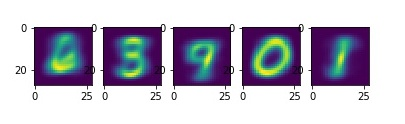
\includegraphics[width=15cm]{MNIST_k05}

$k = 10$\\
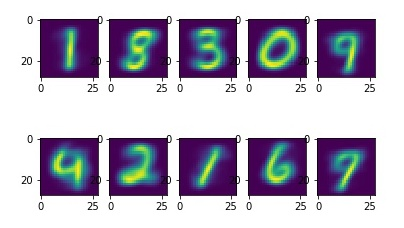
\includegraphics[width=15cm]{MNIST_k10}

\-\\
\-\\
\-\\
$k = 20$\\
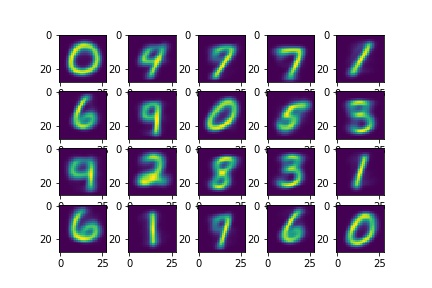
\includegraphics[width=15cm]{MNIST_k20}


It becomes apparent that the resolution of the numbers that are picked out by the clusters improves. For example, it is difficult to identify a number corresponding to the first cluster in the $k=5$ set. In the $k=10$ set we are able to identify most of the numbers (to at least two possible digits) even though not all digits 1-10 are represented. Finally, in the $k=20$ clustering, we have at least one clustering corresponding to each digit 1-10 and the resolution of each cluster is significantly improved.


\newpage
%%%%%%%%%%%%%%%%%%%%%%%%%%%%%%%%%% PROBLEM 2 %%%%%%%%%%%%%%%%%%%%%%%%%%%%%%%%%%
\section*{Problem 2}

\subsection*{\textit{a.})}
\textbf{Low-Rank Approximation: Face Image}

Rank-5, rank-20, and rank 100 approximations:\\
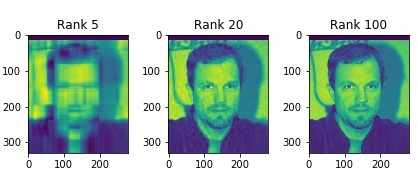
\includegraphics[width=15cm]{face_LRAs}


\subsection*{\textit{b.})}
\textbf{Mean-Squared-Error: Face Image}

Mean-Squared Error for rank-1 through rank-100 approximations of the face image compared to the original.
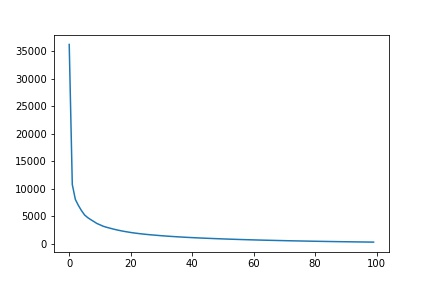
\includegraphics[width=15cm]{face_MSEs}


\subsection*{\textit{c.})}
\textbf{Low-Rank Approximation: Sky Image}

Rank-5, rank-20, and rank 100 approximations:\\
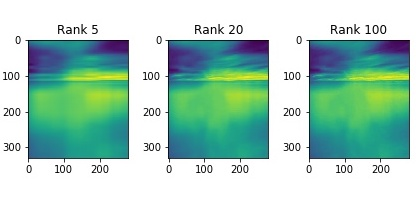
\includegraphics[width=15cm]{sky_LRAs}


\subsection*{\textit{d.})}
For the face image, a rank 40 approximation shows significantly degraded resolution (especially in the forehead area), and a rank 45 approximation still seems a bit fuzzy. I find the rank 50 approximation to be sufficiently close for the two images to be considered identical. (See Jupyter notebook for evidence)

For the sky image, the rank 20 image shows a slight degradation in quality in definition of the colors in the bottom left. This effect is significantly reduced in a rank 25 image, and by a rank 30 approximation, the original and the low-rank image are nearly indistiguishable.

The difference between the sky and face images is likely caused by the level of detail. The sky image has less distinct features, so reducing the rank will likely have less impact on the clarity of each of those features. (Additionally, from a biological perspective, the human brain is incredibly adept at identifying other human faces. Even very slight differences in the face image may trigger the brain to reject the images as identical, whereas it is more apt to overlook those slight differences in the sky image.)

[See Jupyter notebook for evidence]


\end{document}




